\begin{problem}{Ayman and Stairs (Hard Version)}{standard input}{standard output}{1 second}{256 megabytes}

\textbf{The only difference between the two versions of the problem is the constraints on $n$. In this version $n \leq 10^{18}$.}

Ayman likes stairs very much, and does not get tired of making them. His dad brought him $n$ cubes and Ayman wonders what is the maximum length of stairs he can make with them. Can you help him to find that answer?

A sequence of stairs of length $k$ is a succession of $k$ columns made of cubes, where the $1$-st column has $1$ cube, the $2$-nd column has $2$... and so forth until the $k$-th column.

\begin{center}
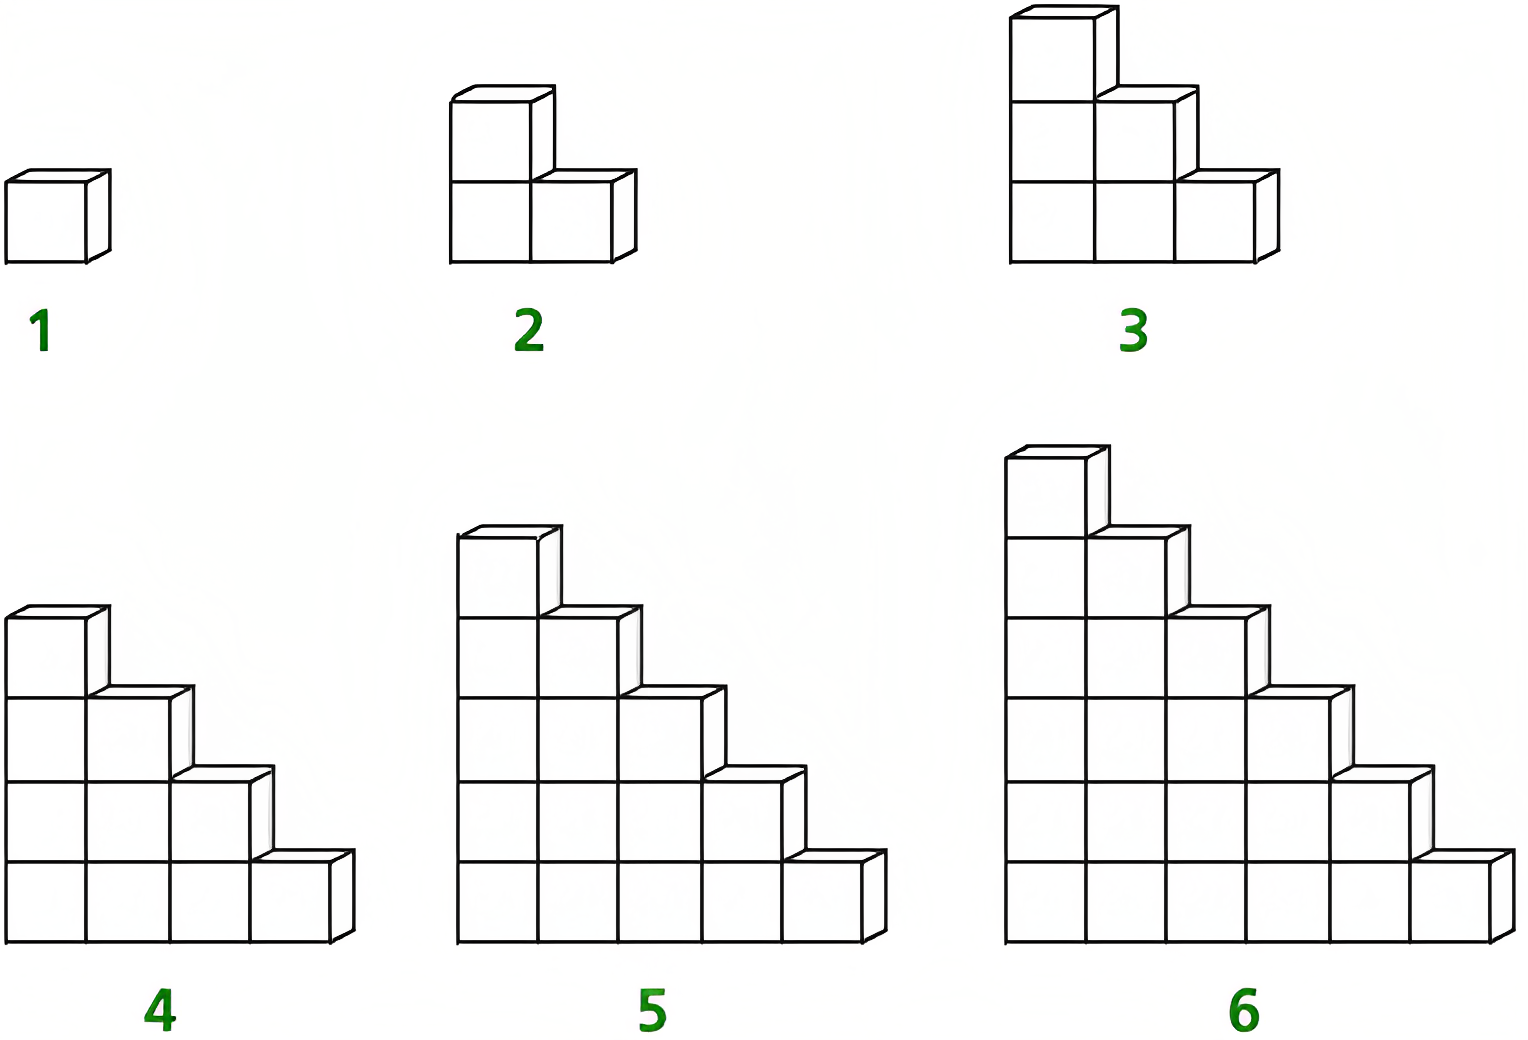
\includegraphics[width=16cm]{figure-1_2.png}
\small{Here is an example of sequences of stairs of lengths from $1$ to $6$}
\end{center}

Note that he does not have to use all the $n$ cubes.

\InputFile
A positive integer $n$ $(1 \leq n \leq 10^{18})$ representing the number of cubes.

\OutputFile
Output one integer, the maximum length of stairs Ayman can make.

\Examples

\begin{example}
\exmpfile{example.01}{example.01.a}%
\exmpfile{example.02}{example.02.a}%
\exmpfile{example.03}{example.03.a}%
\end{example}

\Note
Since the input is large in some testcases, it won't fit into 32-bit integer type, so you should use at least 64-bit integer type in your programming language (like \t{long long} for C/C++).

If you are using C language, you can scan a \t{long long} using \t{scanf("\%llu", &input)}.

\end{problem}

